\documentclass[11pt,letterpaper]{article}
\usepackage[top=1in,bottom=1in,left=1in,right=1in]{geometry}
\usepackage[numbers]{natbib}      % http://merkel.zoneo.net/Latex/natbib.php
\usepackage{lmodern}
\renewcommand\familydefault{\sfdefault} 
\usepackage[T1]{fontenc}

\bibpunct{(}{)}{;}{a}{,}{,}
\usepackage{chngpage}
\usepackage{stmaryrd}
\usepackage{amssymb}
\usepackage{amsmath}
\usepackage{amsthm}
\usepackage{graphicx}
\usepackage{lscape}
\usepackage{subfigure}
\usepackage{parskip}
\usepackage[usenames,dvipsnames]{color}
\usepackage{indentfirst}
\definecolor{myblue}{rgb}{0,0.1,0.6}
\definecolor{mygreen}{rgb}{0,0.3,0.1}
\usepackage[colorlinks=true,linkcolor=black,citecolor=mygreen,urlcolor=myblue]{hyperref}
\newcommand{\bocomment}[1]{\textcolor{Bittersweet}{[#1 -BTO]}}
\newenvironment{itemizesquish}{\begin{list}{\labelitemi}{\setlength{\parskip}{0.6cm}\setlength{\itemsep}{0em}\setlength{\labelwidth}{2em}\setlength{\leftmargin}{\labelwidth}\addtolength{\leftmargin}{\labelsep}}}{\end{list}}
\newcommand{\norm}[1]{\left\lVert#1\right\rVert}
\newcommand{\ignore}[1]{}

\theoremstyle{definition}
\newtheorem{question}{Question}[section]

\setlength{\parindent}{30pt}
\linespread{1}

\title{
   CMSC 701: Final report
}

\author{
	Khanh Nguyen and Ugur Koc
}

\begin{document}
\maketitle

\section{Introduction}

Neighbor-joining is a widely used algorithm for reconstructing phylogenetic trees from evolutionary distance data. The method takes a greedy bottom-up approach, iteratively joining pairs of taxonomic units that minimizes pre-computed distances. In this work, we present our C++ implementation of the algorithm. We compare the running time of the implementation with other popular packages. In addition, we also provide a benchmark on our implementation for computing the distance matrix between sequences. We found that BLAH BLAH.

\section{Methods}

\subsection{Hierarchical clustering}

\subsection{Phylogenetic trees}

\begin{figure}[h]
  \centering
  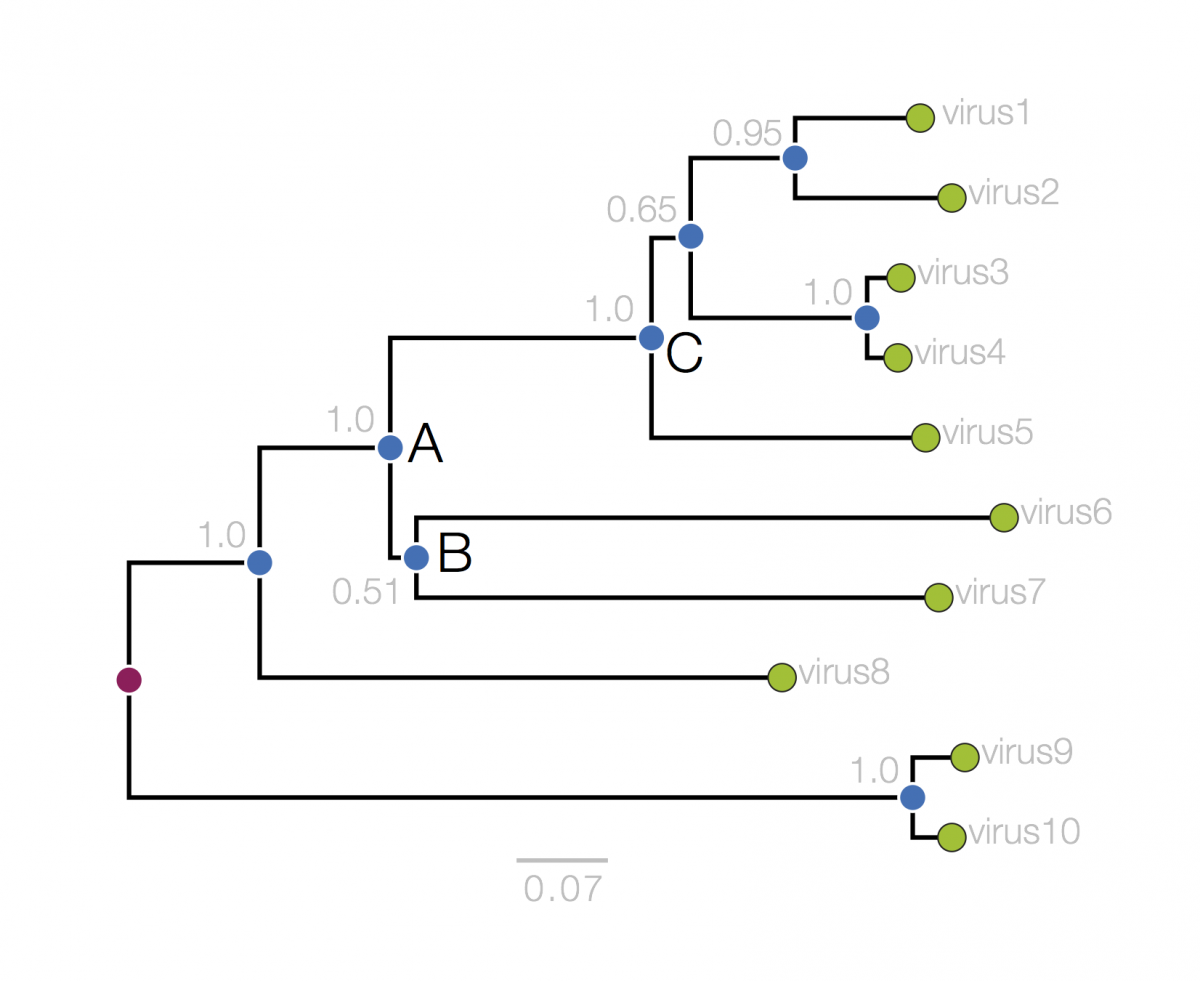
\includegraphics[width=0.6\textwidth]{phylogram_1a.png}
  \caption{An example of phylogenetic tree.}
  \label{fig:phytree}
\end{figure}

Phylogenetic trees are branching diagrams that show the evolutionary relationships between biological species. A weighted phylogenetic tree, with weights associated with its edges, captures the notion of genetic distances between species. Hence, looking at a weighted phygenetic tree, we understand not only \textit{how} but also \textit{how much} they relates or differs from one another. Figure \ref{fig:phytree} \footnote{Image taken from \url{http://epidemic.bio.ed.ac.uk/how_to_read_a_phylogeny}} features a artificial phylogentic tree of 10 viruses. Each virus is represented by a leave in the tree. Each internal node marks a milestone when a genetic divergence occurs. Notice that the lengths of the horizontal lines represents time periods. DFor example, we can see that the divergence between virus 1 and virus 2 occurs before the divergence between virus 3 and 4. Different phylogentic trees may choose to represent different types of genetic distances. In this example, the number assigned to each edge is the proportion of substitutions occuring on a sequence (the number of substituions divided by the length of the sequence). 

\subsection{Neighbor-joining algorithm}

In this report, we consider the problem of constructing a phylogentic tree from a set of protein sequences. From a data mining or machine learning perspective, this problem can be framed as hierarchical clustering problem. There are many approaches to tackle this problem. Although statistical approaches such as maximum likelihood methods have been employed to build complex evolution model, classical approaches such as the neighbor-joining algorithm has the advantage of being easy to implement and scalable to large datasets. Our focus in this report is on the neighbor-joining algorithm (CITE NEIGHBORJOINING). 

TODO: Khanh 
Neigh-joining algorithm takes 


\subsection{Compute distances between sequences}

TODO: Ugur

\section{Experiment}
\subsection{Data}


\subsection{Results}
\subsubsection{Compare with other neighbor-joining implementations}

TODO: Khanh 

\subsubsection{Compare with other distance matrix implementations}

TODO: Ugur

\end{document}






